\chapter{Human Computable Passwords}\label{ch:hcp}
The previous chapter concludes that managing passwords for online accounts has become a major issue for the modern Internet user. It seems to be impossible to remember and maintain enough strong passwords to keep all accounts secured. The scheme presented in this chapter is designed to help users maintain and remember multiple strong passwords, while also protecting these after multiple password breaches. HCP takes advantage of the human brain allowing users to calculate passwords from public challenges, using their own mind to do so. 

\par The HCP scheme is proposed by Blocki et al. \cite{hcp-blocki}. In addition to the scheme itself, the proposal introduces security and usability notions used to analyze the proposed scheme. This chapter describes the scheme as well as associated security and usability concerns. The first section consists of definitions and notations as used by Blocki \cite{hcp-blocki} to describe the scheme. Next, human computable functions are introduced as this is the main component used in the password management scheme. How these functions can be used to generate and memorize unique passwords in practical cases is presented. Finally, usability concerns related to the scheme are reviewed.

\section{Password Management Scheme}
The main idea of the HCP scheme is to have a set of challenges stored in persistent memory, typically on a computer or even a piece of paper. Users then use a mapping and a function to calculate the response to each challenge, which eventually gives the password. It is worth noting that this is different from other "traditional" passwords managers, in that the passwords are not stored, only challenges "helping" users remember passwords. To create a new password, random challenges are generated, users then compute the passwords from these using a memorized secret mapping. To reproduce the password later, the same challenges is displayed to the users, which then can calculate the same password. This procedure is explained further in \autoref{usage}, and in algorithms \ref{auth-algo} and \ref{new-challenge-algo}.

\subsection{Definitions and Notation}
\paragraph{Memory types} considered are either \emph{persistent} or \emph{associative} memory \cite{human-memory}. This project follow the settings of Blocki et al. \cite{naturally-rehearsing, hcp-blocki} where persistent memory are equal to writing something down or somehow storing it reliably, but not securely. When talking about persistent memory, it can be assumed that this is publicly available, or at least that an adversary has undisclosed access to the data. This should be emphasized since this is a strength to the scheme, nothing needs to be kept secret after establishing the needed prerequisites. 
    \par Associative memory is the memory the users, namely their human memory. This memory is different from the persistent memory in that it is totally private but needs to be rehearsed to not lose data. In a password management scheme rehearsing should optimally be part of the natural activity of a user. The best case would be if a user could rehearse and keep all his passwords in associative memory by simply logging in to his accounts as normal. This is a central challenge for all password schemes \cite{naturally-rehearsing}.

The password management scheme uses a random mapping between a set of objects to single digits which has to be memorized by the users. This mapping is denoted as $\sigma : [n] \rightarrow \mathbb{Z}_d$. If $X_k \subseteq [n]^k$ is the space of ordered clauses of $k$ variables, let $C\sim X_k$ be a clause chosen at random from $X_k$. $C$ is now a set of k objects (e.g. $(2,4,7,8)$). Now $\sigma (C) \in \mathbb{Z}_d^k$ is the mapped variables corresponding to challenge $C$. $C$ can consist of any type of object, such as pictures letters or digits, with the mapping $\sigma$ always being to digits.

\begin{example}
    If $\sigma(x) = x+1  \bmod 10$ and $C = (10,25,36)$ then $\sigma(C) = (1,6,7)$.
\end{example}

\par One of these challenges, $C$, is referred to as a \emph{single digit challenge}, which will consist of $k$ ordered objects chosen at random. The function $f: \mathbb{Z}^k_d \rightarrow \mathbb{Z}_d$ is a human computable function as discussed in the next section. Users then responds to a challenge $C$ by computing $f(\sigma(C))$. A complete password challenge, $\vec C = (C_1,\dots,C_t) \in (X_k)^t$ , will consist of $t$ separate, single digit challenges. The response to $\vec C$, namely $f(\sigma(\vec C))$, is the complete password. 
\par The password management scheme works by generating one challenge, $\vec C$, for each of a user's accounts $A_1,\dots,A_m$. The challenges $\vec C_1,\dots,\vec C_m \in (X_k)^t$ are stored in persistent memory. When users want to log in to a service they are shown the challenge corresponding to that account, users then calculate the responses to all the single digit challenges, producing the password.

\subsection{Human Computable Functions}\label{human-func}
At the core of the scheme is a human computable function $f$ and the memorized mapping $\sigma$. The scheme require the composite function of these two $f \circ \sigma$ to be \emph{human computable}, which simply means that the function should be easily computable by the users without aids. To fulfill this requirement the function can't involve many operations, since the complexity and thus computation time would be too high. As shown by Miller \cite{magic-seven_miller}, a human can only store $7 \pm 2$ pieces of information at a given time, on the other hand humans are quite good at simple operations such as addition modulo 10. In example "1+6+5+3+8+9+3+1+4+6+7+7+6 mod 10" would be easy for most humans to compute by simply doing one operation at a time, updating the answer after each addition. With this approach only one piece of information is stored in memory of the users at any time. The problem with such an expression is the amount of terms. 
\par The requirements needed for a function to be human computable can thus be summarized as the following, and formalized in Requirement \ref{human-function-req}:
\begin{itemize}
    \item Can only involve "simple" operations, mainly addition and recalling from long-term memory.
    \item Limited amount of terms.
    \item Limited amount of operations.
\end{itemize}
\begin{remark}
    All operations used in the human computable functions discussed in this project are modulo $10$, as this is the most natural for most humans.
\end{remark}
\begin{requirement}
    \label{human-function-req}
    Function $f$ is said to be $\hat t$-human computable if a human can compute it in his head in $\hat t$ seconds.
\end{requirement}

\par Blocki et al. \cite{hcp-blocki} believe that a function $f$ is human-computable if it can be computed using a fast streaming algorithm, meaning that the input is presented as a sequence of objects that only can be evaluated once. The algorithm would have to be simple since humans are not good at storing intermediate values \cite{magic-seven_miller}. Typical operations fast enough for the human to compute in his head is addition modulo 10 which is natural for most humans to do quickly, and recalling a mapped value $\sigma(i)$ from memory.

\begin{definition}
    \label{ptm-computable}
    A function $f$ is $(P, \tilde t, \tilde m)$-computable if there is a space $\tilde m$ streaming algorithm computing $f$ using $\tilde t$ operations from $P$.
\end{definition}
\begin{remark}
    Space $\tilde m$ means that the algorithm requires no more than $\tilde m$ memory slots during calculation. Slots are typically used for storing values and executing primitive operations such as addition~\cite{space-complexity}.
\end{remark}



\noindent As for the primitive operations in $P$, the following are considered:
\begin{itemize}
    \item \emph{Add} takes two digits $x_1$ and $x_2$, and returns the sum $x_1 + x_2$ mod 10.
    \item \emph{Recall} returns the secret value $\sigma(i)$ corresponding to an input index $i$. The mapping $\sigma$ is memorized by the users, allowing the recall operation to be done quickly in the users' head.
    \item \emph{TableLookup} involves looking up the $x$'th value from a table of 10 indices.
\end{itemize}

\begin{example}
    The function $f \circ \sigma(i_1,\dots,i_5) = \sigma(i_1) + \dots + \sigma(i_5)$ is $(P,9,3)$-computable, since it requires 9 operations from $P$, 5 recall operations and 4 add operations. $\tilde m=3$ since a sequence of additions $i_1 + \dots + i_n$, requires one slot for storing the sum, one slot for storing the next value in the sequence and one slot to execute the addition.
\end{example}

\par Blocki et al.~\cite{hcp-blocki} conjecture that a user $H$ will be able to calculate a $( P, \tilde t, 3 )$-computable function in $\hat t = \gamma_H \tilde t$ seconds. Blocki believes that users with moderate mathematical background should be able to achieve results yielding $\gamma_H \le 1$  This conjecture is part of the experiment presented later in this project. 


\begin{conjecture}\label{conjecture1}
    \cite{hcp-blocki} For each user H there is a small constant $\gamma_H > 0$ such that any $(P,\tilde t, 3)$-computable function $f$ is $\hat t$-human computable with $\hat t = \gamma_H \tilde t$.

\end{conjecture}

\subsection{Secure Human Computable Functions}
Blocki et al. \cite{hcp-blocki} suggest a family of human computable functions defined as follows.
\centerline{ $ f_{k_1,k_2}(x_0,\dots,x_{9+k_1+k_2})= x_j + \mathlarger{\sum}\limits^{9+k_1+k_2}_{i=10+k_1} x_i \quad mod\quad 10,$}\\
\centerline{with $j = \mathlarger{\sum}\limits^{9+k_1}_{i=10} x_i \quad mod \quad 10\quad$ and $\quad k_1>0$, $k_2>0$ }
\vspace{2mm}


\begin{definition}
    \label{f-function}
    $f(x_0,x_2,\dots,x_{13}) = \big( x_{(( x_{11} + x_{10} )\quad mod \quad 10)} + x_{12} + x_{13} \big)\quad mod \quad 10$ 
\end{definition} 

\begin{definition}
    \label{fo-function}
    $f\circ \sigma(x_0,x_2,\dots,x_{13}) = \big(\sigma ( x_{(\sigma(x_{11}) + \sigma(x_{10})\quad mod \quad 10)} ) +\sigma ( x_{12} ) + \sigma( x_{13} )\big)\quad mod \quad 10$ 
\end{definition}

\par This project will use one of these functions, with $k_1=k_2=2$. From now on this will be the function referred to as $f$, the function is defined in definition \ref{f-function}. For an in depth analysis of the function see "Usable Human Authentication: A Quantitative Treatment"~\cite{Blocki2014}. Blocki argues that an adversary would have to see $\tilde \Omega(n^{1.5})$ challenge-response pairs to be able to start recovering the secret mapping $\sigma$. A realistic mapping $\sigma$ would probably consist of no more than 100 object to digit mappings. A secret mapping consisting of $n=100$ mappings would require an attacker to steal 1000 challenge-response pairs (100 accounts given password length of 10) to recover the secret mapping. In practice this might be the tricky part of the scheme, memorizing a mapping of $100$ object-digit mappings might be possible, but probably too hard for a "normal" user to bother doing. It might be more reasonable to use a smaller set of mappings which will lower the security of the scheme, while making it more accessible for novice users. 
\par An example mapping which could be feasible in practice is characters to single digits, with characters from the alphabet and digits between $1$ and $10$. This mapping would yield $n=26$ which would require an attacker to recover significantly less challenge-response pairs. With $n=26$ the amount is down to $133$ compared to the $1000$ with $n=100$. Still, this would require to fully compromise $13$ or more accounts with password lengths of $10$ characters. How many objects $n$ in the mapping function, should be decided after evaluating how many accounts, and how sensitive the information associated are.
\par In addition to $f$, a mapping function $\sigma$ is used. Definition \ref{fo-function} defines the composite function of $f$ and $\sigma$ which is used later in the actual password scheme. The response to a challenge $\vec C$ is calculated using this function $f \circ \sigma$. Figure \ref{pw-flow} and table \ref{defs} summarize how the system works, random challenges are stored persistently in a database and a secret mapping is stored in the associative memory of the users. A challenge is then converted into a password by applying the mapping and a human computable function to each single digit challenge. The combined results of these calculations yield the complete password of the site.



\begin{figure}[ht]
    \centering
    \fbox{ 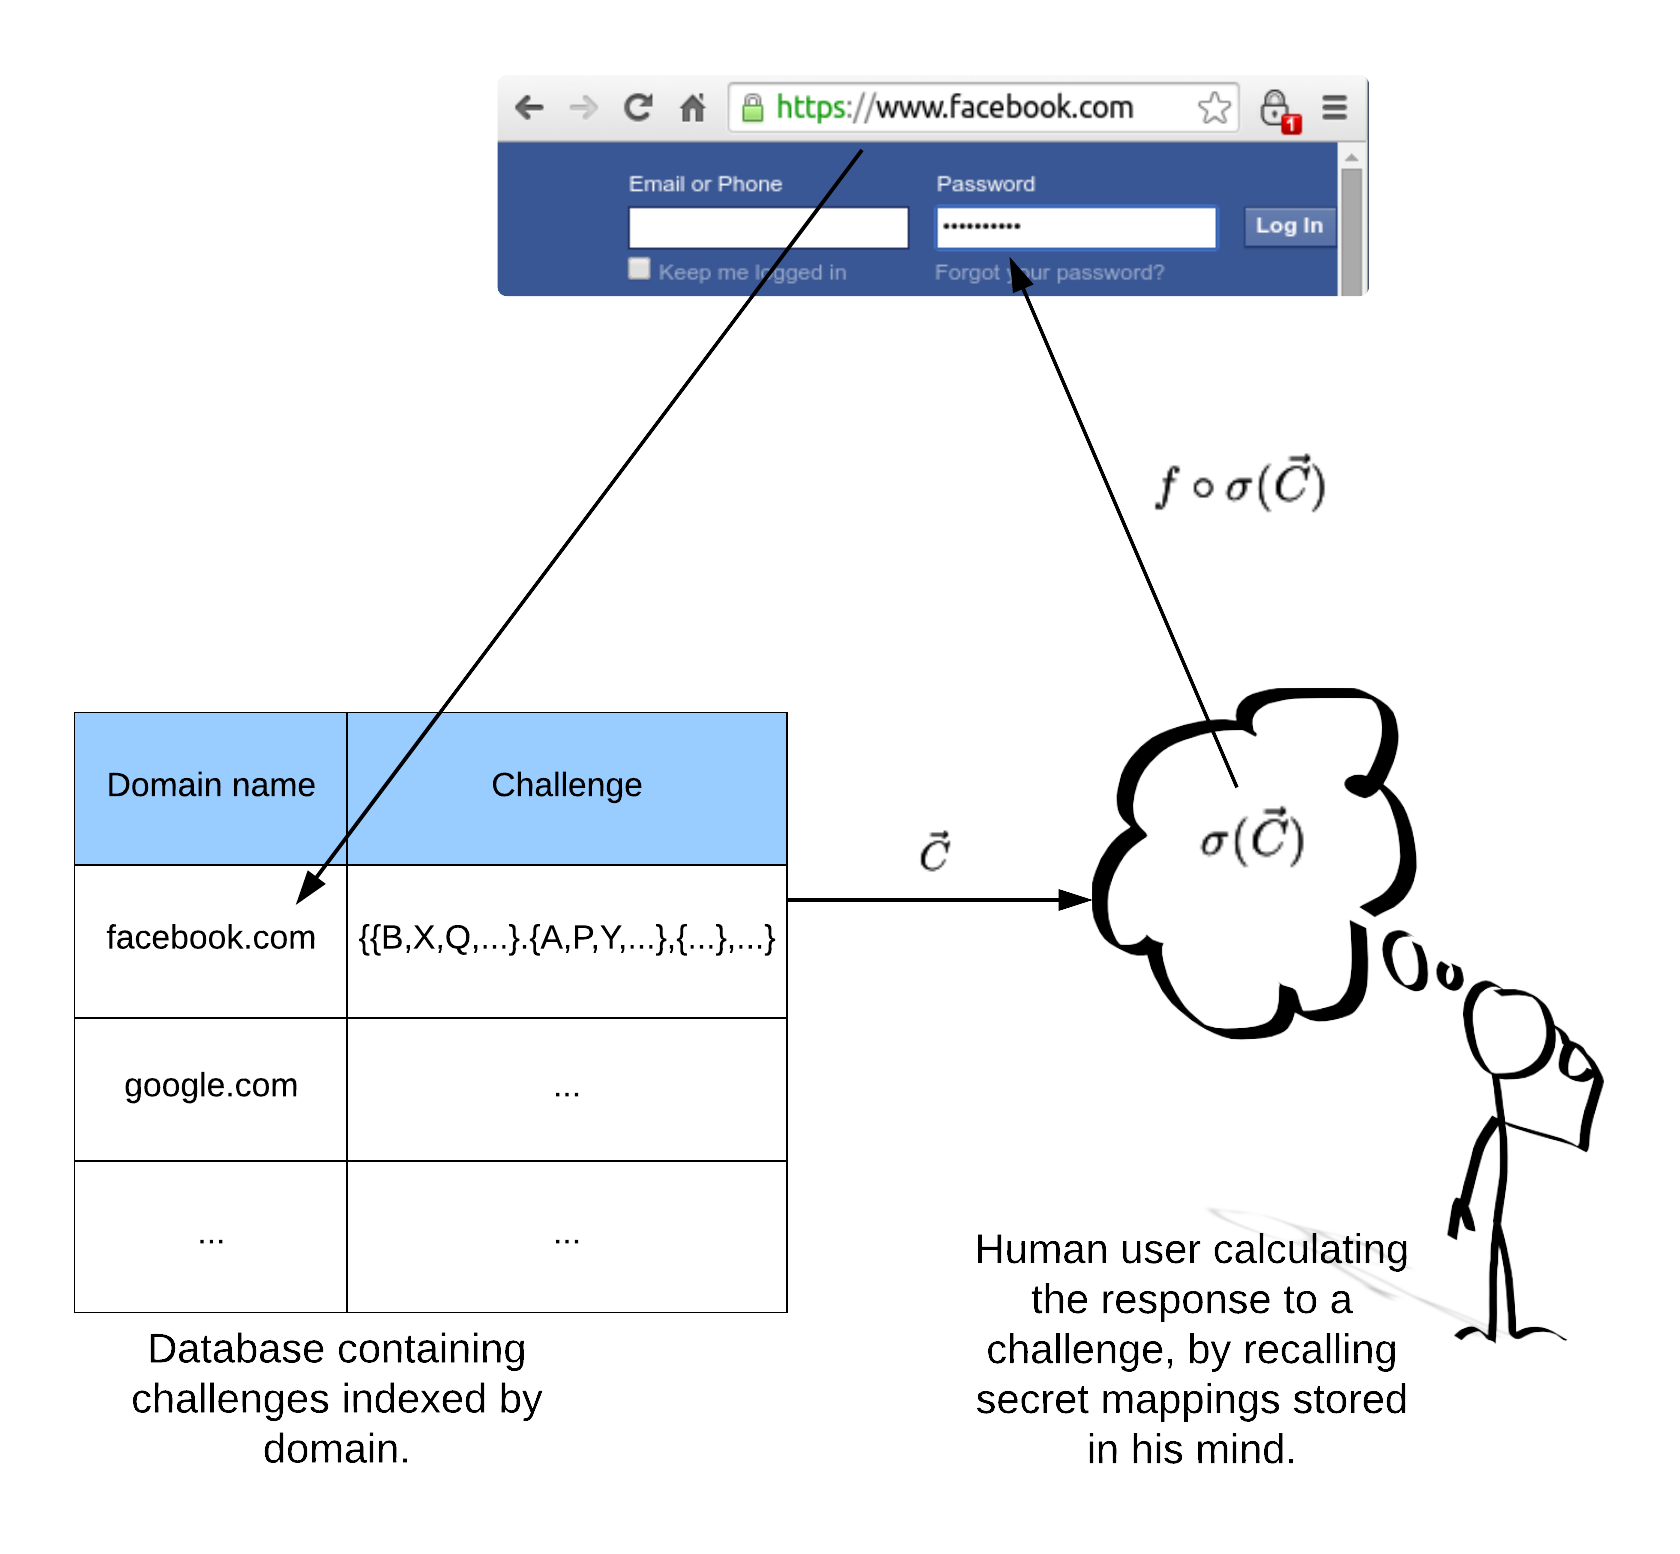
\includegraphics[width=\textwidth]{pw-flow} }
    \caption{The database contains challenges indexed by domain name, which is fetched and displayed to the users. User can then calculate the response to this challenge by using the secret mapping $\sigma$ which is only stored in their minds.}
    \label{pw-flow}
\end{figure}


\begin{table}
    \centering
    \begin{tabular}{ |c|l| }
        \hline
    $f(x_0,\dots,x_{13})$ & \begin{tabular}{@{}l@{}}A human computable function used in the password\\ management scheme investigated in this project.\\ Defined in definition \ref{f-function} \end{tabular}  \\\hline
        
        $\sigma(x)$ & \begin{tabular}{@{}l@{}}Random mapping to be memorized by the users. It takes\\ in an object of some sort and returns a digit between\\ 0 and $d$, $d$ can be assumed to always be $10$. \end{tabular}  \\
        \hline
        $C$ & \begin{tabular}{@{}l@{}}A single digit challenge, this is a challenge consisting of $13$\\ randomly chosen ordered objects. A single digits challenge\\ in this project is a list of $13$ random letters (e.g. ("B", "E", ...)).\\ One of these is used to compute \emph{one} character of a user's\\ password. \end{tabular} \\
        \hline
        $\vec C$ & \begin{tabular}{@{}l@{}}A password challenge, consisting of $t$ single digit challenges.\\ A password challenge yields a complete password after\\ calculating the response to all single digits challenges contained\\ in it. \end{tabular} \\
        \hline
    \end{tabular}
    \caption{Summary of notation.}
    \label{defs}
\end{table}



\subsection{System parameters} \label{sec-params}
\par The previous section has described how the password management scheme works. The most important characteristic that should be emphasized is that there is two possible sources of information leakage in the password management scheme, namely the database used to store the challenges and the different site's password storage. The latter is e.g. the database of facebook.com which usually will consist of salted hashes of the users' passwords. The challenges are, as mentioned, stored in persistent memory, which is assumed to be available to an adversary, so leaking the challenge alone is not necessarily a problem. If password hashes are leaked from online services the password to that exact service might be lost, but the scheme still ensures that no other passwords can be reduced from the compromised password. An adversary attacking the scheme would try to recover the secret mapping $\sigma$ since this would allow him to compute all the passwords of a user using that mapping. Such an attack, if possible, would require a set amount of challenge-response pairs. 
\par There are some interesting trade-offs related to the parameters of the HCP scheme. A bigger set of mappings makes it increasingly hard to recover $\sigma$, but it becomes  harder to memorize and rehearse as well. It is reasonable to say that complexity of a mapping function grows linearly with the number of mappings $n$, and the resistance versus attackers grows polynomially, thus much quicker than the complexity, see \autoref{trade-off1}. In other words, for each mapping added to $\sigma$, $n$ is increased with one and the security multiplied with $1.5$. The trade-off which would have to be evaluated for each user is then how much effort the users are willing to put into memorizing the mappings, versus how secure they want it to be. This should be evaluated in regards to how "important" the passwords and the accompanying accounts are, and how many accounts the users plan on having. It is not worth memorizing a large set of mappings only to store a few passwords, since there would not be enough mappings to "lose" for an adversary to recover even a small mapping set.
\par Another relation is between password length and number of accounts which would have to be stolen. With $n$ mappings, the number of accounts needed to start recovering $\sigma$ is a function of the password length as seen in \autoref{trade-off2}. If the passwords are very long only a few logins would have to be stolen to recover $\sigma$. This is important to take note of since one of the main strengths of the password scheme is that even if one account is compromised all the others are still secure since each site has a different, "unrelated" password. If the revelation of only a few accounts could compromise the secret mapping, all the passwords of the users might be lost.
\par A user requiring very secure passwords might generate very long passwords of $20+$ characters for each of his accounts. If, by chance, the number of mappings was smaller than suggested, all these "strong" passwords might be lost if only a few of them was to be compromised through a password breach. Users are not advised to use short passwords, but the secret mapping needs to be long enough to support the length and number of passwords a user wants to generate using the scheme.

\par The number of accounts needed to recover the mapping can be used as a practical way of describing the security of the scheme, observation \ref{security-param1} defines this parameter as an inequality reliant on the password lengths $x$ and the number of mappings $n$. \autoref{a-var} illustrates the relationship between password lengths and number of mappings needed to achieve different levels of security. How high the parameter $\hat a$ is depends on how long and how many passwords users intend to have. 


\begin{observation}
    \label{security-param1}
    The security of human computable function including a mapping function, $f \circ \sigma$, as defined in definition \ref{fo-function} and \autoref{human-func}, can be described through the expected number of accounts $\hat a$ which needs to be compromised to start recover the secret mapping $\sigma$, given passwords of length $x$ and $n$ mappings in $\sigma$. $\hat a$ is then 
\begin{equation} \hat a < \frac{n^{ 1.5 }}{x} \label{hata} \end{equation}.
    \label{a-theorem}
\end{observation}

\begin{example}
    A user plans on having passwords of length 20 for all of his many important accounts, and wants these to be securely stored even if it requires him to use more time on rehearsal. In this case, assume that a user wants his accounts be secure even if 100 accounts are leaked. Using \autoref{hata} with $x=20$ and $\hat a = 100$, gives $100 < \frac{n^{1.5}}{20} \implies y > 159$. This means that the user would have to memorize at least $159$ unique random mappings to achieve the desired level of security against leakages. By lowering $\hat a$ to 50, which still is strong, the user would only have to memorize  \\
    If users were to save only a few shorter passwords, for example requiring only security allowing loss of $20$ accounts and passwords of length $15$, they would need to memorize at least $45$ mappings. \\
    Using this formula users would have to evaluate how many mappings are realistic to memorize. 
\end{example}

\begin{figure}
\begin{tikzpicture}
    \begin{axis}[axis lines = left, xlabel=$n$]
    \addplot[domain=0:10, samples=10, color=red]{x^1.5};
    \addlegendentry{$n^{1.5}$};
    \addplot[domain=0:10, samples=3, color=blue]{x};
    \addlegendentry{$n$};
\end{axis}
\end{tikzpicture}
\caption{Number of challenge-response pairs required to recover mapping $\sigma$ as a function of the size of the mapping $n$. }
\label{trade-off1}
\end{figure}

\begin{figure}
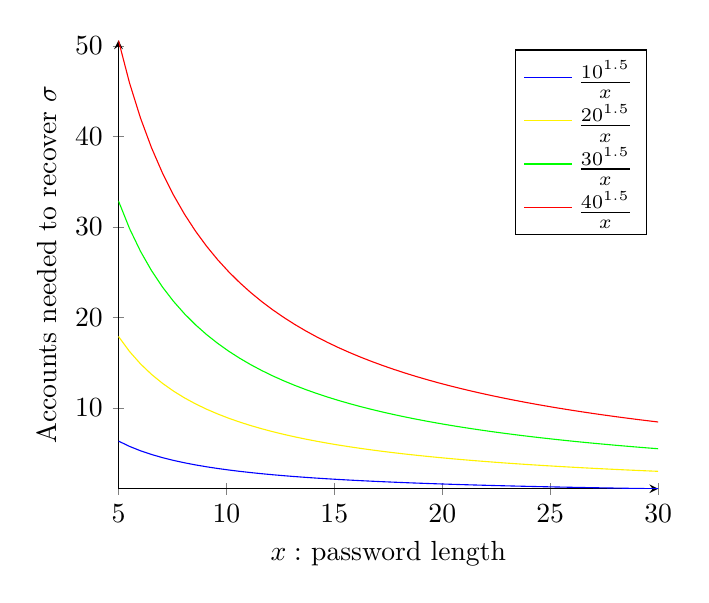
\begin{tikzpicture}
    \begin{axis}[axis lines = left, xlabel=$x: $ password length, ylabel=Accounts needed to recover $\sigma$]
    \addplot[domain=5:30, samples=50, color=blue]{(10^1.5)/x};
    \addlegendentry{$\frac{10^{1.5}}{x}$};
    
    \addplot[domain=5:30, samples=50, color=yellow]{(20^1.5)/x};
    \addlegendentry{$\frac{20^{1.5}}{x}$};
   
    \addplot[domain=5:30, samples=50, color=green]{(30^1.5)/x};
    \addlegendentry{$\frac{30^{1.5}}{x}$};
   
    \addplot[domain=5:30, samples=50, color=red]{(40^1.5)/x};
    \addlegendentry{$\frac{40^{1.5}}{x}$};
\end{axis}
\end{tikzpicture}
\caption{Number of accounts needed to recover the mapping $\sigma$.}
\label{trade-off2}
\end{figure}


\begin{figure}
\begin{tikzpicture}
    \begin{axis}[axis lines = left, xlabel= Password length $x$, ylabel=Number of mappings $n$, ymin=0, ymax=200]
   
    \addplot+[name path=A, color=blue, domain=3:30, samples=20, no markers]{(100*x)^(2/3)};
    \addlegendentry[blue]{$\hat a = 100 <  \frac{n^{1.5}}{x}$};

    \addplot+[name path=B, color=red, domain=3:30, samples=20, no markers]{(50*x)^(2/3)};
    \addlegendentry[red]{$\hat a = 50 <  \frac{n^{1.5}}{x}$};

    \addplot+[name path=C, color=green, domain=3:30, samples=20, no markers]{(20*x)^(2/3)};
    \addlegendentry[green]{$\hat a = 20 <  \frac{n^{1.5}}{x}$};

    \addplot+[name path=X, domain=3:30, samples=2, no markers]{200};
    \addplot[blue!30] fill between [of=A and X];
    \addplot[red!30] fill between [of=B and A];
    \addplot[green!30] fill between [of=C and B];
\end{axis}
\end{tikzpicture}
\caption{Inequality plot of 3 different values for $\hat a$}
\label{a-var}
\end{figure}





\section{Practical Usage}\label{usage}
This section will illustrate how a HCP scheme works in practice, using the principles described in the previous sections. Before using the scheme a user have to go through a setup procedure involving memorization of a randomly generated mapping as well as setting up all accounts with passwords calculated from challenges. Section \ref{sec-params} discussed how the scheme can be tweaked to fit different needs a user may have, depending on the required level of security and the amount of accounts and passwords a user may have. A summary of the setup and authentication procedures are presented next.
\subsection{Setup procedure.}
\begin{enumerate}
    \item A secret mapping is the first prerequisite required before the scheme can be used. A random mapping of length $n$ is generated from a set of objects chosen by the users, to digits in $\{0,1,\dots,d\}$. User will typically choose what type of objects to use, this can be an alphabet or a user chosen set of pictures. A system will then choose $n$ of these objects and assign a random digit between $0$ and $d$, $d$ is normally $10$. Algorithm \ref{gen-mapping} shows how the mapping would be generate from a set of objects by assigning random digits to each object. Remember that this mapping function is supposed to only be stored in the memory of the users, and can thus not be evaluated anywhere else than in the mind of that user.
    \item Memorization of the mapping is the next, and most costly procedure. Users basically have to learn the mappings by heart, and be comfortable they will not forget it. After memorizing, the mapping is deleted and not stored anywhere else than in the mind of the users. After finishing this step, there is no way to recover the mapping if users forget it. This might seem like a barrier, but the fact is that the memorization is a one time cost for many users. Active users will naturally rehearse and thus not forget their mapping as long as they keep using the scheme and regularly calculate passwords.
    \item Passwords can now be generated for all the users' accounts. Algorithm~\ref{new-challenge-algo} describes the process of creating a new password for an account. 
    \begin{enumerate}
        \item First users chose the desired length of the password, $t$, to be generated. 
        \item $t$ random challenges are generated and shown one by one to the users, which calculates the responses to these. Each of the responses are one character in the new password. 
        \item The calculated password is then sent to the server typically through a "change password"-form. 
    \end{enumerate}
    \item the same procedure (1-3) can be done for all the accounts users want to include in the password scheme.
\end{enumerate}

\begin{algorithm}
    \caption{Generate mapping $\sigma$.}
    \begin{algorithmic}[1]
        \Require
            \Statex \begin{itemize}
                \item A base $d$.
                \item $O_1,\dots,O_n$ objects, typically letters or pictures.
            \end{itemize}
        
        \For{$i=1 \rightarrow n$}
            \State $k \sim \{0,d\}$
            \State $\vec S \leftarrow (O_i,k)$
        \EndFor
        \Statex

        \Function{$\sigma$}{$O_x$}
            \State search($O_x\quad in\quad \vec S$)
            \State \Return $(O_x, i)$
        \EndFunction
        \Statex
        \State \Return $\sigma$
    \end{algorithmic}
    \label{gen-mapping}
\end{algorithm}
\subsection{Authentication procedure.}\label{subsec:auth}
\begin{enumerate}
    \item Authenticating with a site, which password was previously generated using the scheme, start of by selecting the correct site. The corresponding challenges will then be displayed starting with the first one.
    \item Users calculate the response to each challenge, the same way they did when generating the password. If the calculations are done correctly, the result should be the same.
    \item After calculating the response to all $t$ challenges, the password can be submitted to the server which checks if the hashed value is the same as the stored one. If it is, the user is authenticated.
\end{enumerate}

\begin{remark}
    The notation $f(\sigma(\vec C))$ as used in the algorithms is equal to the composite function $f \circ \sigma(x_0,\dots,x_{13})$ as used in definition \ref{fo-function}.

\end{remark}

\begin{algorithm}
    \caption{Create new challenge for account $A_j \in (A_1,\dots, A_m)$}
    \begin{algorithmic}[1]
        \Require
            \Statex \begin{itemize}
                \item $t$ desired length of password.
                \item $\sigma$ secret mapping memorized by the user.
                \item $f$ a human computable function.
                \item $O_1,\dots,O_n$ objects, typically letters or pictures.
            \end{itemize}
            
        
        \For{$i=1 \rightarrow t$}
            \State $k \sim [0, n] $
            \State $\vec C_i \leftarrow \{O_k\}^{14} $
        \EndFor
        \Statex
        \State $\vec C \leftarrow (\vec C_1,\dots, \vec C_t) $

        \State \textbf{(User)} Computes $(p_1,\dots,p_t)=f(\sigma(\vec C))$
        \State \textbf{(Server)} Store $h_j = H(p_1,\dots,p_t)$
        \State
        \State \Return $\vec C$
    \end{algorithmic}
    \label{new-challenge-algo}
\end{algorithm}


\begin{algorithm}
    \caption{Authentication process for account $A_j \in (A_1,\dots,A_m)$}
    \begin{algorithmic}[1]
        \Require
            \Statex \begin{itemize}
                \item Account $A_j \in (A_1,\dots, A_m)$
                \item Challenges $\vec C = (\vec C_1,\dots,\vec C_t)$ from account $A_j$.
                \item Hash $h_j$ and hash function $H$.
            \end{itemize}

            \For{$i=1 \rightarrow t$}
                \State Display $C_i$ to the user
                \State \textbf{User} Compute $p_i \leftarrow f(\sigma(C_i))$
                \State
                \Comment $p_i$ is the $i$'th character of the password for account $A$
            \EndFor

            \State $\vec P = (p_1,\dots,p_t)$
            \If{$h_j =H (\vec P )$}
            \Comment \textbf{(Server)} 
                \State Authenticated on account $A_j$
            \Else 
                \State Authentication failed
            \EndIf

    \end{algorithmic}
    \label{auth-algo}
\end{algorithm}



\section{Usability}\label{sec:usability}
Blocki et al. \cite{hcp-blocki} consider three usability parameters defining the usability of a human computable function, namely \emph{calculation time}, \emph{memorizing $\sigma$} and \emph{rehearsing $\sigma$}. In addition to these, another influencing factor is introduced, \emph{failure rate}. This section will discuss these requirements and how to influence them.
\begin{itemize}
    \item The effort required to memorize the secret mapping.
    \item The extra rehearsal required of the users to not forget the secret mapping. 
    \item How long it takes a human user to calculate the responses to a set of challenges, eventually producing the password. 
    \item How reliably a human user can calculate password without mistakes.
\end{itemize}
All of these requirements might limit the usability of the scheme, and are thus worth discussing, but this project will focus mostly one the last two requirements, related to computation time and failure rates. These parameters will later be tested through implementing the scheme as a web app and having participants try it out while timing their efforts. 

\subsection{Memorizing the secret mapping.}
As seen in the previous section, a user have to memorize a random mapping from object to digits before starting to use the scheme. This is most likely the biggest and most frightening barrier for any user considering to use the scheme. There are several techniques supposed to help memorizing relations easier, examples are the method of loci \cite{human-memory} which is supposed to enhance memory by visualization. Mnemonic helpers showing objects merged together might help memorize relations as in the case of this project. Blocki et al. \cite{hcp-blocki} propose using mnemonic helpers if the mapping consist of letters to digits. These helpers would typically be a set of pictures showing a visual transition from a letter to a digit. This way might make it easier for users to remember it instead of only being shown "A=1" etc. Some user might also feel that it is easier to memorize other things than letters, such as pictures. Users might even get to choose the set of pictures to be used themselves as long as the corresponding digits are chosen at random. 

\subsection{Rehearsing the secret mapping.}
After memorizing the mappings, the users will have to rehearse it frequent enough to not forget it. Blocki et al. \cite{naturally-rehearsing} defines a model estimating the cost of this rehearsal, the model is described in \autoref{sec:usability-model}. Applying this model to the password management scheme gives insight to how much different types of users have to rehearse. The model predicts how long a user will remember a association between $i$ and corresponding mapping $\sigma(i)$ without further rehearsal. If users are about to forget a mapping according to the predictions, they should be reminded of this. Recall theorem \ref{ERt} and table \ref{users} from \autoref{sec:usability-model}. The formula for $E(ER_t)$ can be used to predict how many extra rehearsals different types of users will be required to do within a given period. \autoref{extra-rehearsals} shows the expected number of extra rehearsals required by the different types of user given the length of the mapping function $n$, during the first year. It is computed using theorem \ref{ERt} with $t=365$ and visitation schedules $\lambda_i$ from each user type as seen in table \ref{users}. For each account $A_i$ a set of public challenges $\vec C_i \in (X_{14})^{10}$ are chosen at random using algorithm \ref{new-challenge-algo}. The expanding rehearsal assumption as defined in \ref{ER} is used, which assumes that for each rehearsal $i$ users does not have to rehearse again for $2^{is}$ units of time. The variable $s$ represents differences between user in terms of memory strength, this experiment uses $s=1$. The values in table \ref{extra-rehearsals} are calculated by generating $100$ samples of $\vec C_i \in (X_{14})^{10}$, then calculating the average expected number of extra rehearsals required by the different user types. $n$ is the number of mappings in $\sigma$.

\begin{table}
    \centering
    \begin{tabular}{ |l|c|c|c| }
        \hline
        User & $n=100$ & $n=50$ & $n=30$ \\
        \hline \hline
        Very Active & $0.396$ & $0.001$ & $\approx 0$ \\
        \hline
        Typical & $2.14$ & $0.039$ & $\approx 0$ \\
        \hline
        Occasional & $2.50$ & $0.053$ & $\approx 0 $  \\
        \hline
        Infrequent & $70.7$ & $22.3$ & $6.1$ \\
        \hline

    \end{tabular}
    \caption{\cite{hcp-blocki} Extra rehearsals required of the users during the first year to remember $\sigma$. Calculated using definition \ref{ERt} with $t=365$ and visitation schedules as in table \ref{users}.}
    \label{extra-rehearsals}
\end{table}

\par The results in table \ref{extra-rehearsals} clearly demonstrates that the HCP scheme does not require much rehearsal at all if used frequently. In fact, for very active, typical and occasional users, memorizing the mapping is a one time cost. After memorizing it at the beginning, using the scheme will provide enough natural rehearsal to maintain the mapping in memory. 
When users compute the response to a challenge $\vec C$ as described in \autoref{subsec:auth}, they will have to recall the mapping of up to $5$ ($(\sigma(x_{11}), \sigma(x_{10}), \sigma(x_{12}), \sigma(x_{13}),\sigma(x_j)$, see definition \ref{fo-function}) values of $i$ for each character of the password. A password length of $10$ would yield recalling, and thus rehearsing, $50$ values of $i$. The same trade-off as discussed in \autoref{sec-params} can be observed here. The more complex the mapping is (larger values of $n$), the more effort is required when memorizing, but no extra rehearsals are necessary even with a larger number of mappings.

    \subsection{Computation Time and Failure Rates.}\label{computation-time}
The final requirement which may limit the usability of the scheme is calculation time. If a user can not compute the response to a challenge correctly in a reasonably short amount of time the scheme would not be usable. How much time a user can tolerate is of course individual, but a too long computation time will directly effect the usability. In addition to the time spent calculating, it is important that the users are able to consistently compute the correct responses. If the failure rate is too high, in respect to the password length, the scheme will not function at all. It is thus more important to have a low enough failure rate than a short calculation time.


\subsubsection{Improving Usability.}\label{improving-usab}

\par To make the computation as easy as possible the challenges would have to be presented to the users in a practical way, facilitating fast and reliable calculation. Using the human computable function from definition \ref{fo-function}, a challenge $C = (x_0, x_1,\dots, x_{13})$ could be displayed as shown in \autoref{challenges}. \\ 
\centerline{ $f\circ \sigma(x_0,x_2,\dots,x_{13}) =$} \\
\centerline{$\big(\underbrace{\sigma ( x_{ (\underbrace{\sigma(x_{11}) + \sigma(x_{10}) )\quad mod \quad 10}_\text{Step 1, 2, \& 3}} )}_\text{Step 4 \& 5} \underbrace{ +\sigma ( x_{12} ) + \sigma( x_{13} )\big)\quad mod \quad 10 }_\text{Step 6 \& 7}$ }. 

To evaluate a challenge using this function and the layout template from \autoref{challenges} a user goes through the following steps:
\begin{enumerate}
    \item Recall the mapping $x_{10}$
    \item Recall the mapping $x_{11}$ 
    \item Add the values from the two previous steps $i = \sigma(x_{10}) + \sigma(x_{11})$.
    \item Locate the element $x_i$ from the table.
    \item Recall the mapping $\sigma(x_i)$.
    \item Recall the mapping $\sigma(x_{12})$ and add this to the previous value, $z = \sigma(x_i) + \sigma(x_{12})$.
    \item Finally recall the mapping $\sigma(x_{13})$ and add it to the previous value, obtaining the final sum $y = z + \sigma(x_{13})$k.
    \item $y$ is the response to the challenge $C$.
\end{enumerate}


\begin{table}[h]
    \centering
    \begin{tabular}{|c c|c|c|}
        \hline
        $x_{10}$ & $x_{11}$ & $x_{12}$ & $x_{13}$ \\
        \hline \hline
        \multicolumn{2}{|c|}{$0:x_0$} & \multicolumn{2}{|c|}{$5:x_5$}\\
        \multicolumn{2}{|c|}{$1:x_1$} & \multicolumn{2}{|c|}{$6:x_6$}\\
        \multicolumn{2}{|c|}{$2:x_2$} & \multicolumn{2}{|c|}{$7:x_7$}\\
        \multicolumn{2}{|c|}{$3:x_3$} & \multicolumn{2}{|c|}{$8:x_8$}\\
        \multicolumn{2}{|c|}{$4:x_4$} & \multicolumn{2}{|c|}{$9:x_9$}\\
        \hline 
    \end{tabular}
    \caption{Layout template for displaying challenges.}
    \label{challenges}
\end{table}


\par Each step depends on at most two earlier steps, allowing users to do the calculation without having to store more than two values in memory at any time. After finishing steps 1-3 they will only keep one value in memory, the previous intermediate results are now irrelevant and can be forgotten. 

\begin{example}
    \autoref{challenge-example} shows the same layout using example objects. The example challenge is $C = \{A, B, C, D, E, F, G, H, I, J, K, L, M, N\}$. Let the mapping function $\sigma$ be the position in the alphabet $\bmod 10$, $\sigma(A)=1, \sigma(B)=2, \sigma(J)=0$ etc. The evaluation of this challenge would be the following.
    \begin{enumerate}
        \item $\sigma(K) = 1$, $\sigma(L)=2$ (K is the $11$th letter in the alphabet, thus $11 \bmod 10 = 1$)
        \item $(11 + 12) \bmod 10 = 3$
        \item $x_3 = D$
        \item $\sigma(D) = 4$ , $\sigma(M)=3$, $\sigma(N)=4$
        \item $(4 + 3 + 4) \bmod 10 = \underline{\underline{1}}$

    \end{enumerate}

    
    \begin{table}[h]
        \centering
        \begin{tabular}{|c c|c|c|}
            \hline
            $K$ & $L$ & $M$ & $N$ \\
            \hline \hline
            \multicolumn{2}{|c|}{$0:A$} & \multicolumn{2}{|c|}{$5:F$}\\
            \multicolumn{2}{|c|}{$1:B$} & \multicolumn{2}{|c|}{$6:G$}\\
            \multicolumn{2}{|c|}{$2:C$} & \multicolumn{2}{|c|}{$7:H$}\\
            \multicolumn{2}{|c|}{$3:D$} & \multicolumn{2}{|c|}{$8:I$}\\
            \multicolumn{2}{|c|}{$4:E$} & \multicolumn{2}{|c|}{$9:J$}\\
            \hline 
        \end{tabular}
        \caption{Layout template for displaying challenges.}
        \label{challenge-example}
    \end{table}


\end{example}

\paragraph{Classification of accounts.}
\autoref{classification} discussed how different accounts should be treated differently depending on the consequences of compromise of the accounts. This can be utilized to limit the number of single digit challenges a user needs to calculate when logging into each account. When adding an account to the system users will have to classify the account in terms of how big consequences a breach would have. This way the users are in control of how much effort is spent calculating passwords versus how strong the passwords are. This will essentially lower both the average total calculation time and attempts needed to calculate each password. 

\par This chapter has presented the ideas behind the HCP management scheme. It has shown how the scheme works with a secret mapping memorized by the users and a human computable function, which together allow users to compute passwords from challenges stored in persistent memory. Algorithms describing the procedures has been shown and described, as well as discussing the usability challenges of such a scheme.
